\section*{Цель работы. }
\addcontentsline{toc}{section}{Цель работы.}

\begin{itemize}
    \item Получение передаточной характеристики, зависимости сопротивления канала полевого транзистора от напряжения затвор-исток и семейства выходных характеристик полевого транзистора.
    \item Расчёт схемы автоматического смещения полевого транзистора.
\end{itemize}

\section*{Исходные данные. }
\addcontentsline{toc}{section}{Исходные данные.}

Транзистор - BSC042N03MS, $U_\text{np}$ = 4 В, $R_\text{n}$ = 220 Ом.


\section*{Рабочее задание. }
\addcontentsline{toc}{section}{Рабочее задание.}
\subsection*{Получение передаточной характеристики полевого транзистора в схеме с общим истоком. }
\addcontentsline{toc}{subsection}{Получение передаточной характеристики полевого транзистора в схеме с общим истоком.}
Собираем схему по заданию:
\begin{figure}[H]
    \centering
    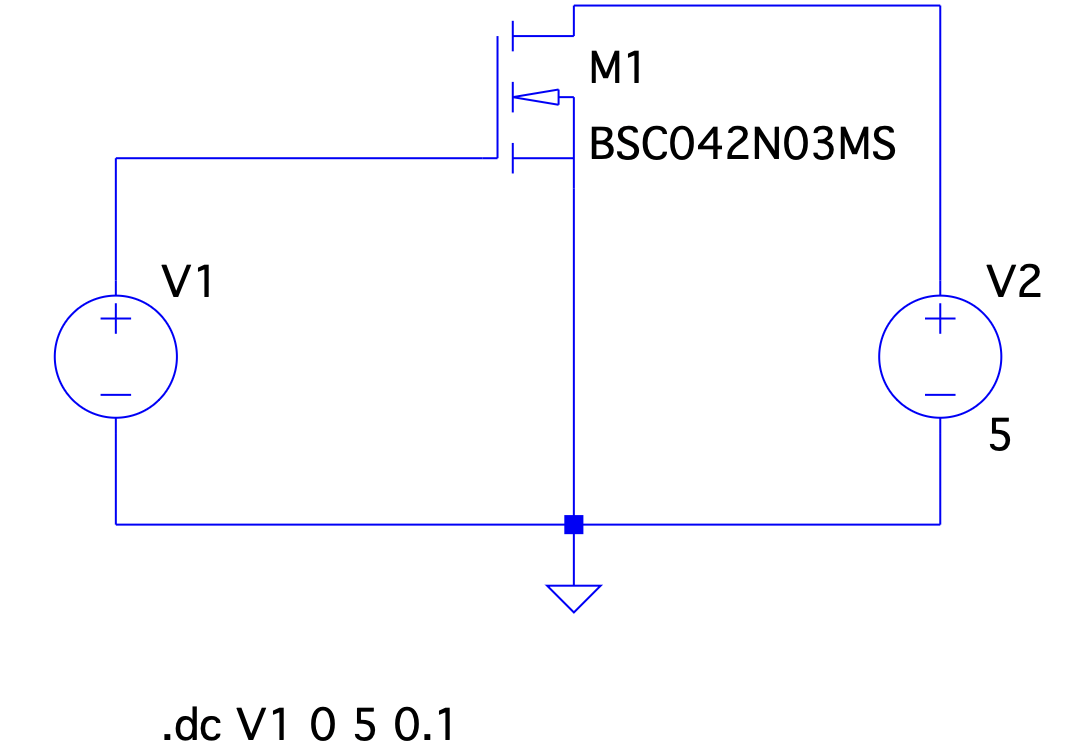
\includegraphics[width=0.6\textwidth]{images/scheme1.png}
    \caption{Схема включения полевого транзистора с общим истоком.}
    \label{fig:hy}
\end{figure}

\newpage
Теперь была получена передаточная характеристика полевого транзистора.

\begin{figure}[H]
    \centering
    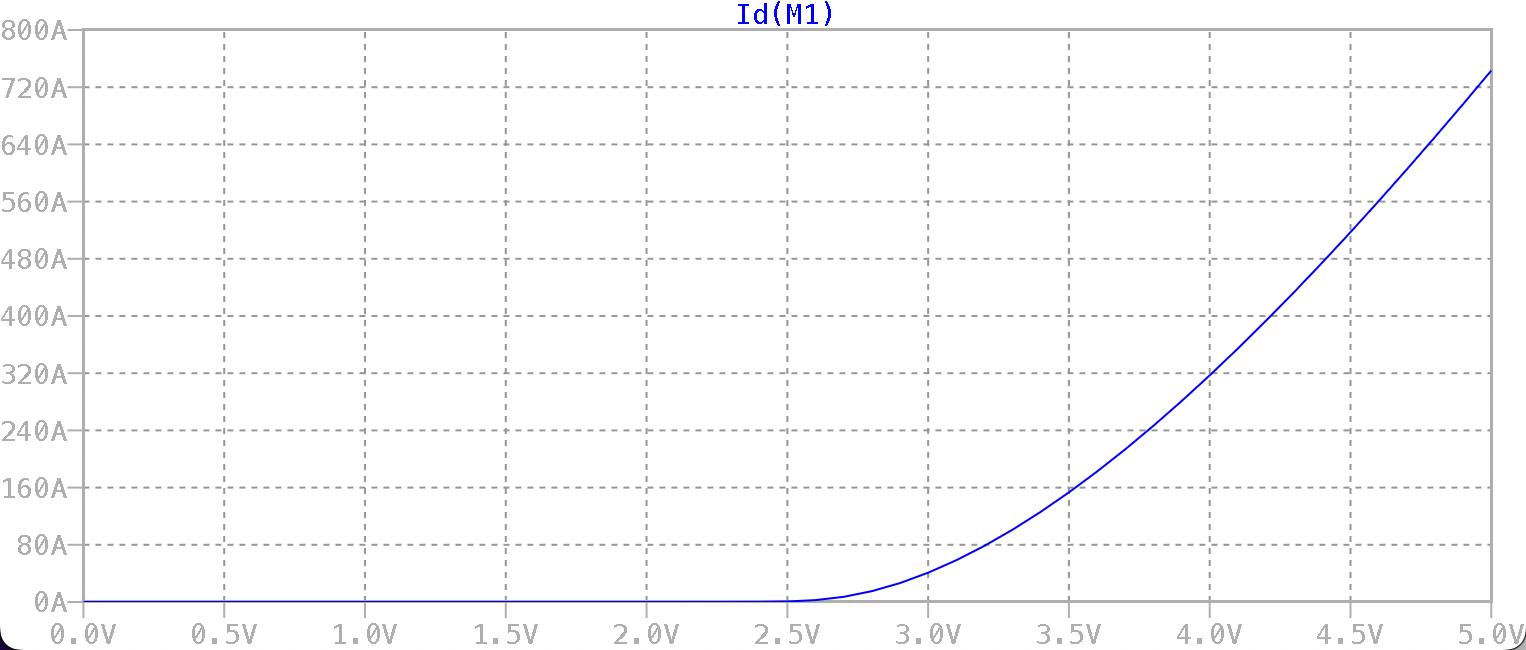
\includegraphics[width=1\textwidth]{images/TC1.png}
    \caption{передаточная характеристика.}
    \label{fig:image}
\end{figure}

Исходя из рисунка №2 пороговое напряжение затвор-исток $U_\text{por} = 2.5 B$ 


Пары точек для расчета крутизны:
\begin{center}
    \item $I_\text{c1} = 160A $,  $U_\text{c1} = 3.5 B$ 
    \item $I_\text{c2} = 320A $,  $U_\text{c2} = 4.0 B$ 
\end{center}


\subsubsection*{Определение крутизны передаточной характеристики}

Крутизна передаточной характеристики определяется по формуле:
$$
S = \frac{I_\text{C2}-I_\text{C1}}{U_\text{ЗИ2}-U_\text{ЗИ1}}.
$$


Подставляя численные значения, получаем:
$$
S = \frac{320-160}{4.0-3.5}
  = \frac{160}{0.5}
  = 320~\text{мА/В}.
$$

Итого:
$$
S = 320~\text{мА/В}.
$$

\subsubsection*{Определение удельной крутизны}

Удельная крутизна полевого транзистора определяется по формуле:
$$
b = \frac{S}{U_\text{ЗИ}-U_\text{пор}},
$$
где $U_\text{пор}=2.5~\text{В}$, а напряжение затвор--исток принимается равным среднему:
$$
U_\text{ЗИ}=\frac{U_\text{ЗИ2}+U_\text{ЗИ1}}{2}.
$$

Вычислим $U_\text{ЗИ}$:
$$
U_\text{ЗИ}=\frac{4.0+3.5}{2}=3.75~\text{В}.
$$

Тогда:
$$
b=\frac{320}{3.75-2.5}
 =\frac{320}{1.25}
 =256~\text{мА/В}^2.
$$

Итого:
$$
b = 256~\text{мА/В}^2.
$$

\subsection*{Получение семейства выходных характеристик полевого транзистора в схеме с общем истоком. }
\addcontentsline{toc}{subsection}{Получение семейства выходных характеристик полевого транзистора в схеме с общем истоком.}
Для снятия выходных характеристик использовалась та же схема, что и в первой части.
Сопоставляем какому напряжению затвор исток соответстсвует каждая из характеристик. Сопоставим их по цвету:

\begin{figure}[H]
    \centering
    
\includegraphics[width=1\textwidth]{images/2.png}
    \caption{Семейство выходных характеристик полевого транзистора.}
    \label{fig:5}
\end{figure}

Теперь для каждой выходной характеристики определеним значение тока стока:
\begin{table}[H]
\centering
\begin{tabular}{|c|c|}
\hline
$U$, В & $I_\text{C}$, А \\ \hline
2.5 & 0.92 \\ \hline
2.9 & 29.31 \\ \hline
3.3 & 110 \\ \hline
3.7 & 227 \\ \hline
4 & 340 \\ \hline
\end{tabular}
\end{table}

Теперь рассчитаем значение крутизны для каждой характеристики.

\begin{table}[H]
\centering
\begin{tabular}{|c|c|c|}
\hline
$U$, В & $I_\text{C}$, мА & $S=\sqrt{2bI_\text{C}}$, мА/В \\ \hline
2.5 & 0.92  & 21.7  \\ \hline
2.9 & 29.31 & 122.5 \\ \hline
3.3 & 110   & 237.3 \\ \hline
3.7 & 227   & 340.9 \\ \hline
4.0 & 340   & 417.2 \\ \hline
\end{tabular}
\end{table}

\subsection*{Расчёт усилительного каскада на полевом транзисторе.}
\addcontentsline{toc}{subsection}{Расчёт усилительного каскада на полевом транзисторе.}


\textbf{Расчёт параметров режима}\\

\begin{enumerate}
    \item \textbf{Выходная мощность на нагрузке:}
    $$
    P_\text{ВЫХ} = \frac{U_\text{Hm}^2}{2 R_H} = \frac{4^2}{2 \cdot 220} = \frac{16}{440} \approx 0.0364\ \text{Вт} = 36.4\ \text{мВт}
    $$
    
    \item \textbf{Максимальный ток через нагрузку:}
    $$
    I_\text{Hm} = \frac{U_\text{Hm}}{R_H} = \frac{4}{220} \approx 0.01818\ \text{А} = 18.18\ \text{мА}
    $$
    
    \item \textbf{Сопротивление в цепи стока $R_C$:}
    Выбираем $R_C = 0.3 \cdot R_Н$:
    $$
    R_C = 0.3 \cdot 220 = 66\ \text{Ом}
    $$
    Принимаем стандартное значение $R_C = 68$ Ом.
    
    \item \textbf{Максимальный амплитудный ток стока:}\\
    Эквивалентное сопротивление параллельного соединения:
    $$
    R_\text{экв} = R_C \parallel R_Н = \frac{R_C \cdot R_H}{R_C + R_H} = \frac{68 \cdot 220}{68 + 220} \approx 51.94\ \text{Ом}
    $$
    Тогда:
    $$
    I_\text{Сm} = \frac{U_\text{Hm}}{R_\text{экв}} = \frac{4}{51.94} \approx 0.077\ \text{А} = 77\ \text{мА}
    $$
    
    \item \textbf{Ток стока в режиме покоя:}
    $$
    I_\text{С0} = 1.5 \cdot I_\text{Сm} = 1.5 \cdot 0.077 \approx 0.1155\ \text{А} = 115.5\ \text{мА}
    $$
    
    \item \textbf{Напряжение сток-исток в режиме покоя:}
    $$
    U_\text{СИ0} = 1.2 \cdot U_\text{Hm} + |U_\text{ПОР}| = 1.2 \cdot 4 + 2.5 = 4.8 + 2.5 = 7.3\ \text{В}
    $$
    
    \item \textbf{Напряжение источника питания:}
    $$
    U_\text{П} \geq U_\text{СИ0} + I_\text{С0} R_C = 7.3 + 0.1155 \cdot 68 \approx 7.3 + 7.854 = 15.154\ \text{В}
    $$
    Округляем до большего стандартного значения: $U_\text{П} = 16$ В.
    
    \item \textbf{Уточнение напряжения сток-исток покоя:}
    $$
    U_\text{СИ0} = U_\text{П} - I_\text{С0} R_C = 16 - 0.1155 \cdot 68 \approx 16 - 7.854 = 8.146\ \text{В}
    $$
    Проверяем условие:
    $$
    U_\text{СИ0} > U_\text{Hm} + |U_\text{ПОР}| = 4 + 2.5 = 6.5\ \text{В} \quad \text{✓ выполняется}
    $$
\end{enumerate}

\textbf{Определение напряжения смещения на затворе}\\

Для тока покоя $I_\text{С0} = 0.1155$ А используем аппроксимацию передаточной характеристики:
$$
I_\text{С} = b (U_\text{ЗИ} - U_\text{ПОР})^2
$$
Подставляем значения:
$$
0.1155 = 0.256 \cdot (U_\text{ЗИ0} - 2.5)^2
$$
Решаем относительно $U_\text{ЗИ0}$:
$$
(U_\text{ЗИ0} - 2.5)^2 = \frac{0.1155}{0.256} \approx 0.4512
$$
$$
U_\text{ЗИ0} - 2.5 \approx 0.6717
$$
$$
U_\text{ЗИ0} \approx 3.17\ \text{В}
$$

\textbf{Построение статической линии нагрузки (СЛН)}\\

\begin{figure}[H]
    \centering
    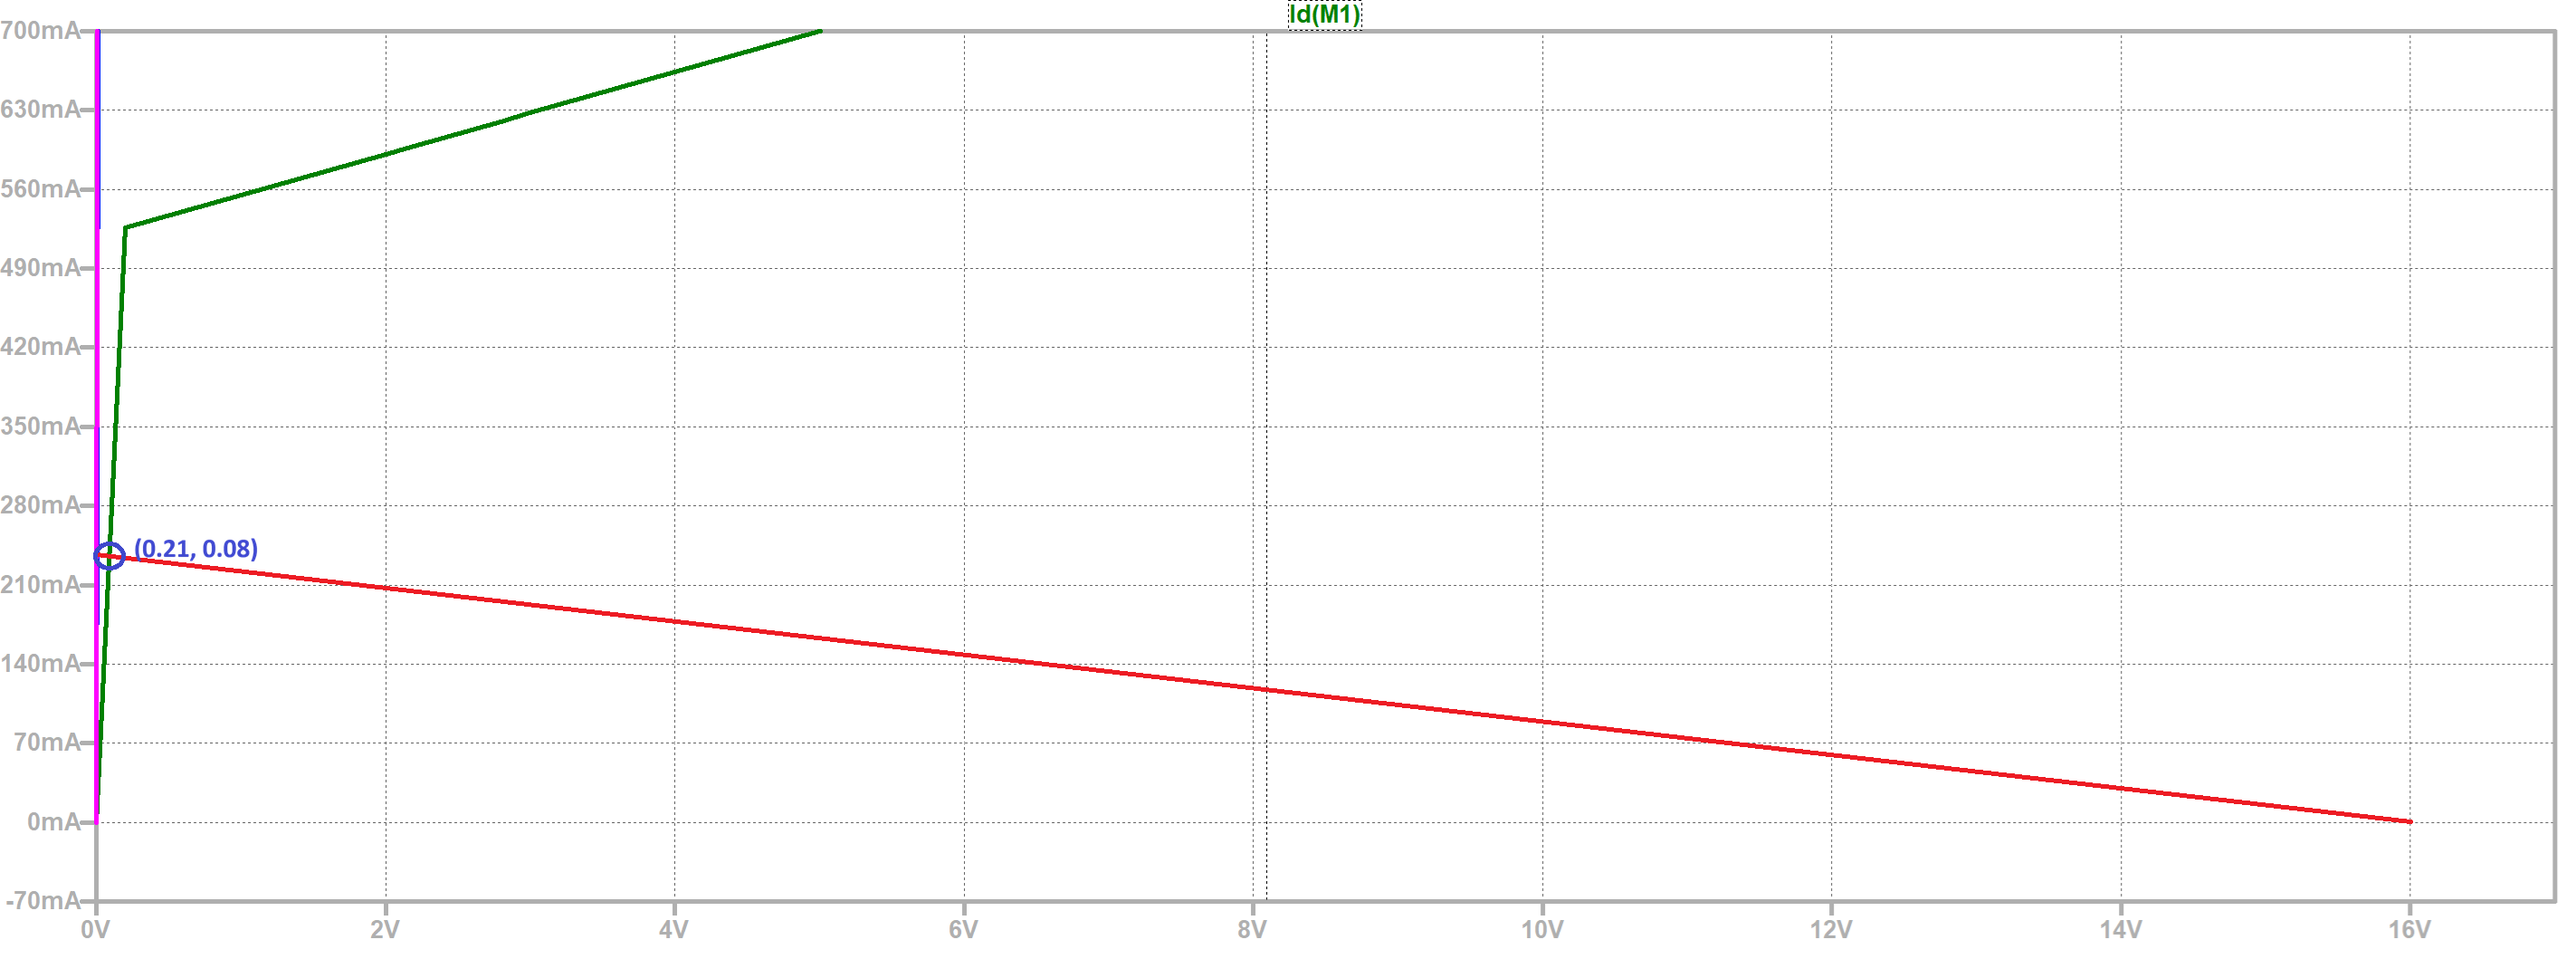
\includegraphics[width=1\textwidth]{images/nagline.png}
    \caption{Нагрузочная линия}
    \label{fig:fd}
\end{figure}

На семействе выходных характеристик отмечаем:
\begin{itemize}
    \item Исходную рабочую точку (И.Р.Т) с координатами $(U_\text{СИ0} = 8.15\ \text{В},\ I_\text{С0} = 0.1155\ \text{А})$
    \item Точку на оси напряжений: $(U_\text{П} = 16\ \text{В},\ I_\text{С} = 0)$
\end{itemize}

Соединяем эти точки прямой — это СЛН. Точка пересечения СЛН с осью токов определяет максимально возможный ток стока:
$$
I_\text{Сmax} = \frac{U_\text{П}}{R_C} = \frac{16}{68} \approx 0.235\ \text{А}
$$

\textbf{Проверка условий безопасной работы транзистора}\\

Используем предельные параметры для BSC042N03MS:
\begin{itemize}
    \item Максимальное напряжение сток-исток: $U_\text{СИmax.доп} = 30$ В
    \item Максимальный ток стока: $I_\text{Сmax.доп} = 40$ А
    \item Максимальная мощность рассеивания: $P_\text{Сmax.доп} = 33$ Вт
\end{itemize}

Проверяем:
\begin{enumerate}
    \item $U_\text{СИmax.доп} = 30\ \text{В} > U_\text{П} = 16\ \text{В}$
    \item $I_\text{Сmax.доп} = 40\ \text{А} > I_\text{Сmax} = 0.235\ \text{А}$
    \item $P_\text{Сmax.доп} = 33\ \text{Вт} > U_\text{СИ0} I_\text{С0} = 8.15 \cdot 0.1155 \approx 0.941\ \text{Вт}$
\end{enumerate}

Все условия соблюдаются, режим выбран корректно.

\textbf{Расчёт цепей смещения}\\

В схеме с общим истоком напряжение на затворе задаётся делителем $R_1$ и $R_2$. Поскольку исток соединён с землёй, то $U_\text{ЗИ0} = U_З$. Выбираем сопротивление параллельного соединения резисторов делителя:
$$
R_1 \parallel R_2 = 1\ \text{МОм}
$$

Рассчитываем номиналы резисторов:
$$
R_1 = \frac{U_\text{П}}{U_\text{ЗИ0}} \cdot (R_1 \parallel R_2) = \frac{16}{3.17} \cdot 1 \approx 5.05\ \text{МОм}
$$
Принимаем стандартное значение $R_1 = 5.1$ МОм.

$$
R_2 = \frac{U_\text{ЗИ0}}{U_\text{П} - U_\text{ЗИ0}} \cdot R_1 = \frac{3.17}{16 - 3.17} \cdot 5.1 \approx \frac{3.17}{12.83} \cdot 5.1 \approx 1.26\ \text{МОм}
$$
Принимаем $R_2 = 1.3$ МОм.

Проверяем эквивалентное сопротивление:
$$
R_1 \parallel R_2 = \frac{5.1 \cdot 1.3}{5.1 + 1.3} \approx \frac{6.63}{6.4} \approx 1.036\ \text{МОм}
$$
что близко к выбранному значению.

\textbf{Выбор разделительных конденсаторов}\\

Ёмкости конденсаторов $C_1$ и $C_2$ выбираем из условия бесперебойного прохождения усиливаемого сигнала:
$$
C_1 = C_2 = 1\ \text{мкФ}
$$

\textbf{Итоговые параметры рассчитанного усилительного каскада}\\

\begin{table}[H]
\centering
\begin{tabular}{|l|c|}
\hline
\textbf{Параметр} & \textbf{Значение} \\ \hline
Напряжение питания $U_\text{П}$ & 16 В \\ \hline
Резистор в цепи стока $R_C$ & 68 Ом \\ \hline
Резисторы делителя $R_1$ & 5.1 МОм \\ \hline
Резисторы делителя $R_2$ & 1.3 МОм \\ \hline
Разделительные конденсаторы $C_1, C_2$ & 1 мкФ \\ \hline
Выходная мощность $P_\text{ВЫХ}$ & 36.4 мВт \\ \hline
Ток покоя стока $I_\text{С0}$ & 115.5 мА \\ \hline
Напряжение покоя сток-исток $U_\text{СИ0}$ & 8.15 В \\ \hline
Напряжение смещения затвора $U_\text{ЗИ0}$ & 3.17 В \\ \hline
\end{tabular}
\end{table}


\textbf{Моделирование работы схемы при постоянном входном сигнале.}\\
\begin{figure}[H]
    \centering
    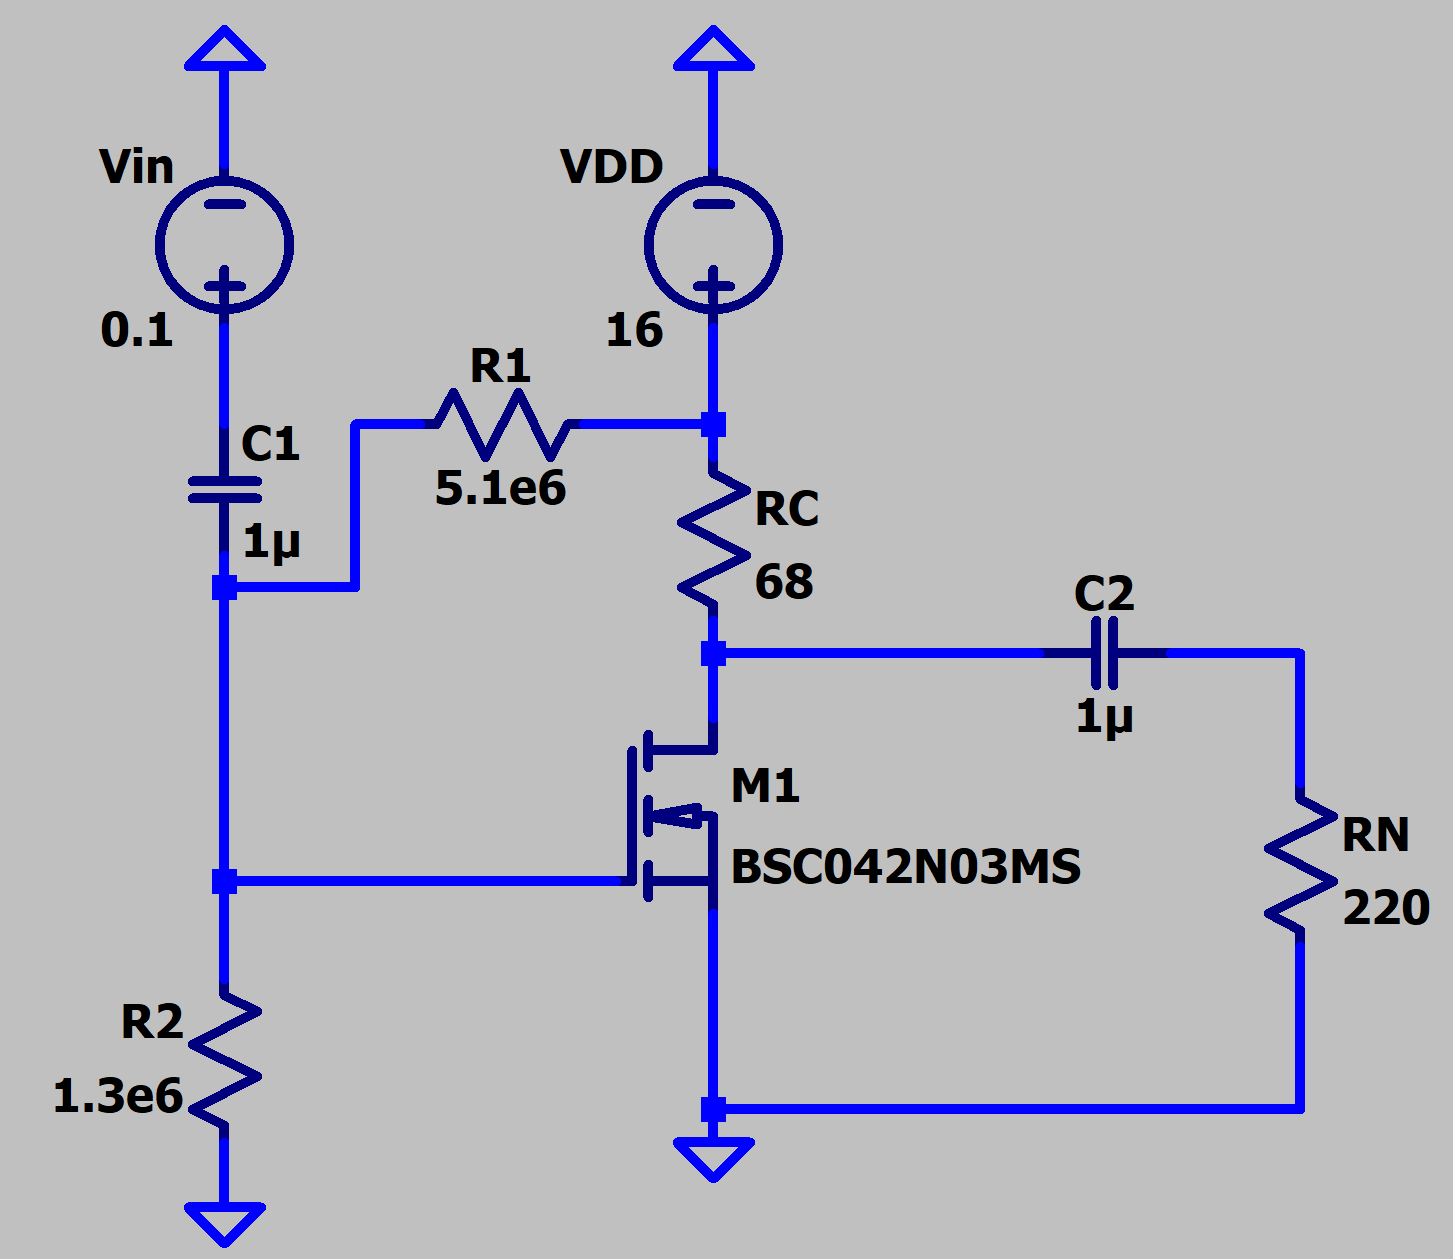
\includegraphics[width=0.5\textwidth]{images/scheme3.png}
    \caption{Схема}
    \label{fig:s}
\end{figure}
Моделирование представлено на рис. \ref{fig:а}
\begin{figure}[H]
    \centering
    
\includegraphics[width=1\textwidth]{images/3.png}
    \caption{Осциллограммы выходного сигнала}
    \label{fig:а}
\end{figure}
\begin{figure}[H]
    \centering
    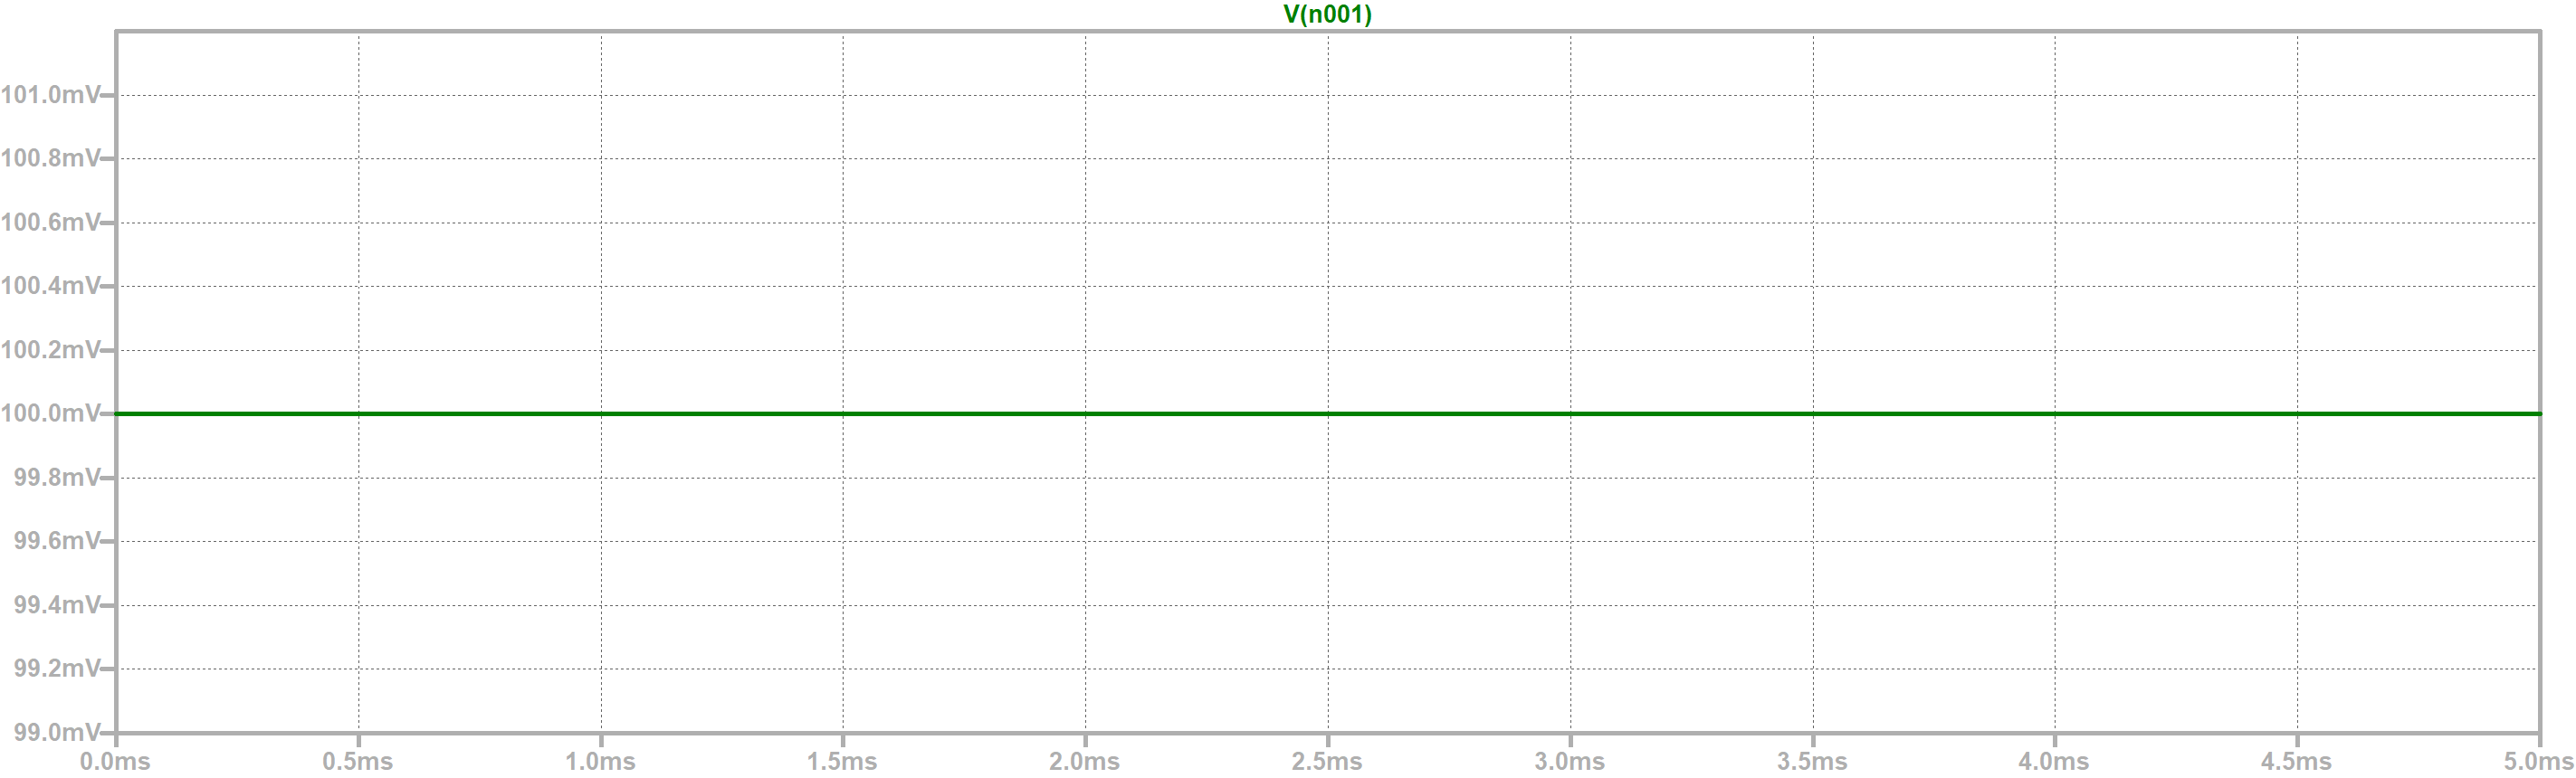
\includegraphics[width=1\textwidth]{images/o.png}
    \caption{Входной сигнал}
    \label{fig:kiа}
\end{figure}

Видим, что при постоянном входном сигнале ток и напряжение отсутствуют, т.к. конденсаторы разрывают цепь.\\


\textbf{Моделирование работы схемы при гармоническом входном сигнале.}\\
Моделирование представлено на рис. \ref{fig:kа}
\begin{figure}[H]
    \centering
    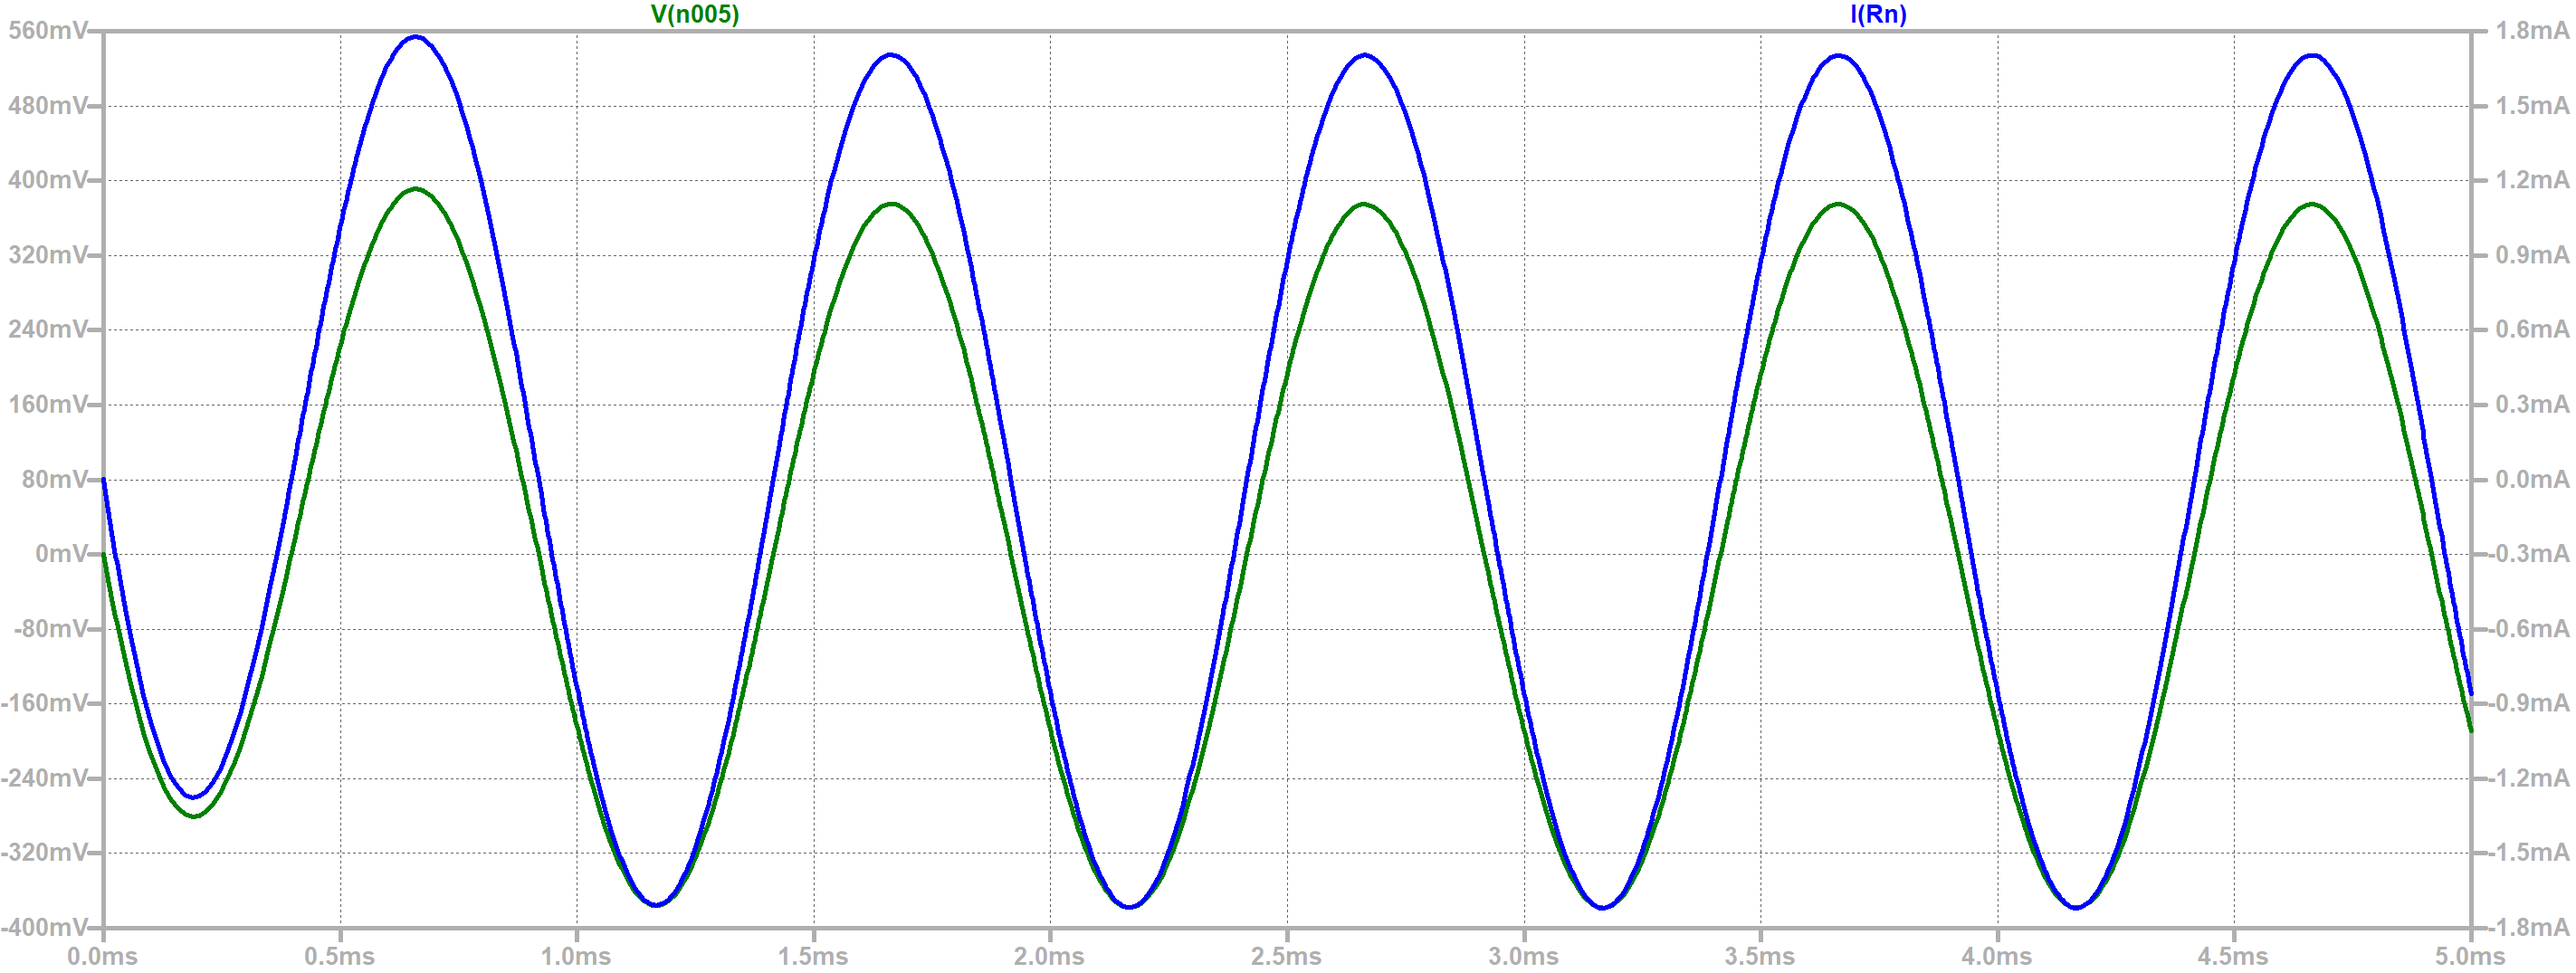
\includegraphics[width=1\textwidth]{images/q.png}
    \caption{Осциллограммы выходного сигнала}
    \label{fig:kа}
\end{figure}
\begin{figure}[H]
    \centering
    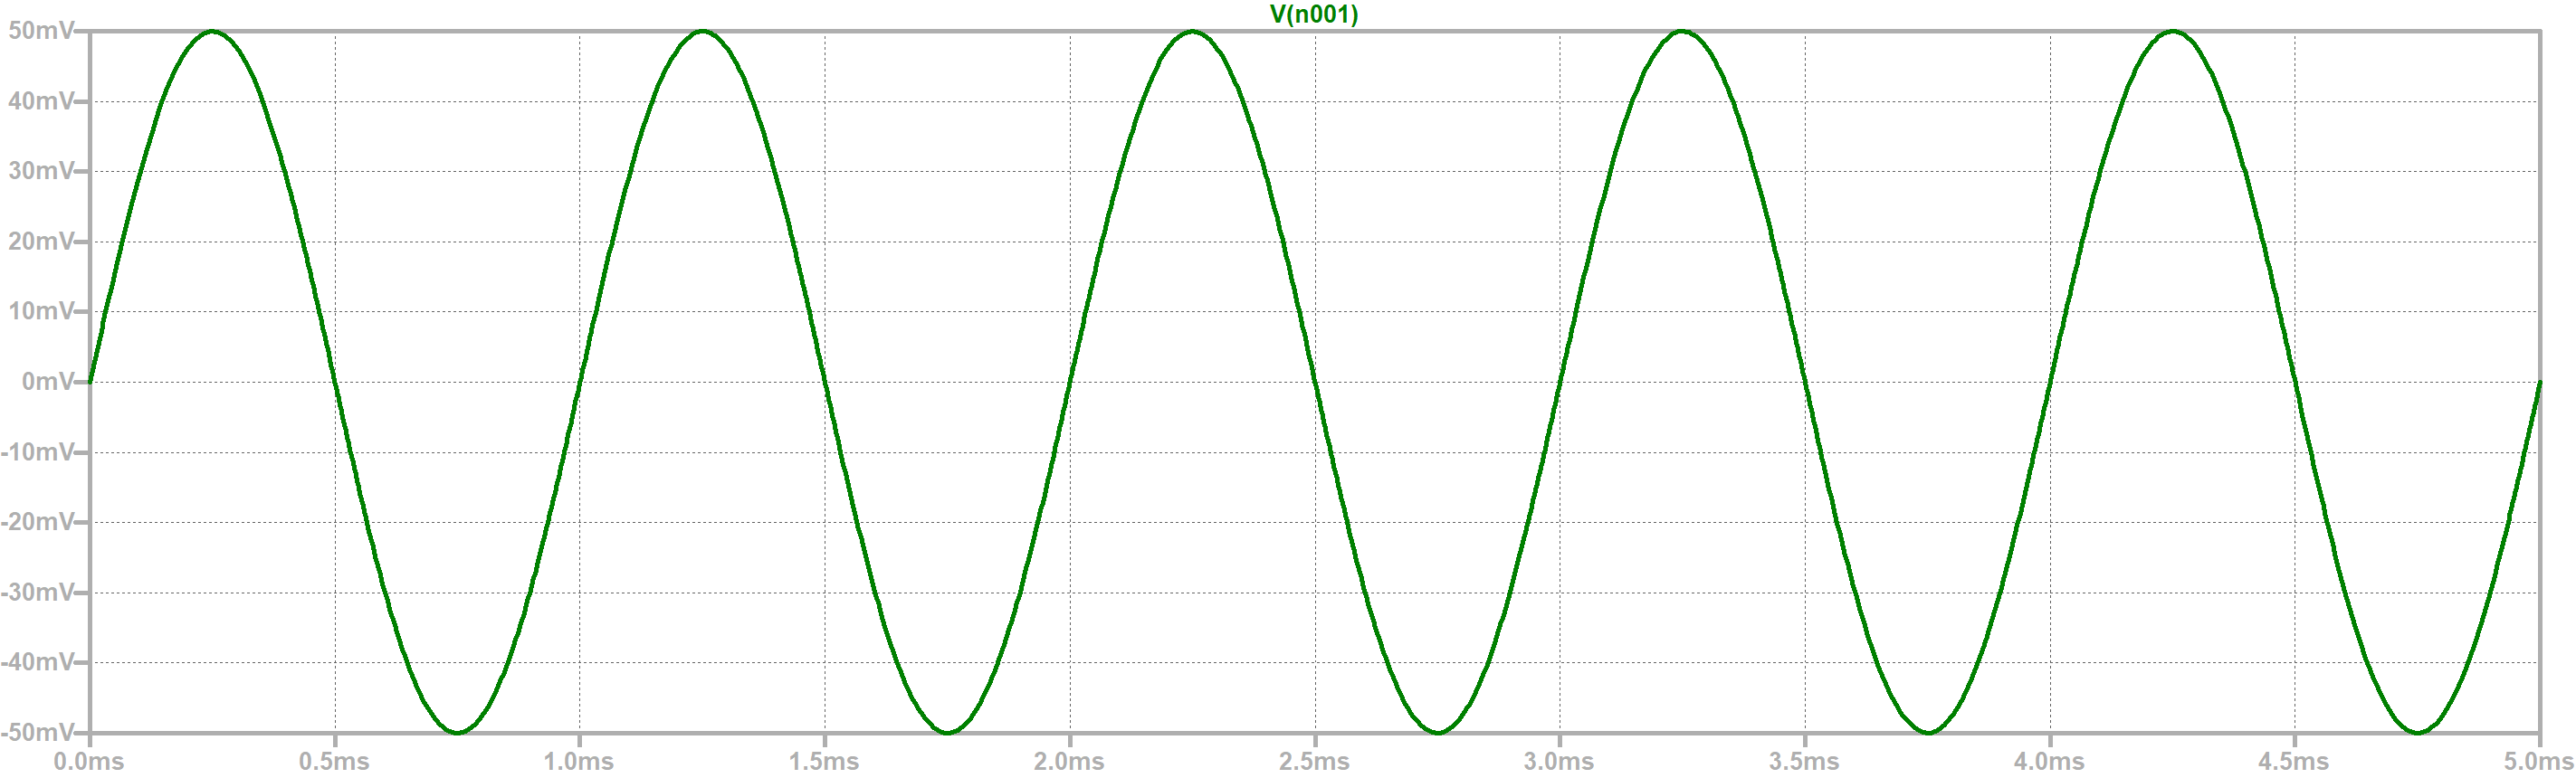
\includegraphics[width=1\textwidth]{images/j.png}
    \caption{Входной сигнал}
    \label{fig:kаl}
\end{figure}
Коэффициент усиления по напряжению $K_U$ рассчитывается как отношение амплитуды выходного напряжения к амплитуде входного напряжения:

\[
K = \frac{U_{\text{вых.амп}}}{U_{\text{вх.амп}}}=\frac{380}{50}=7.6
\]
\section*{Выводы}
\addcontentsline{toc}{section}{Выводы}

В ходе лабораторной работы были экспериментально сняты статические характеристики полевого транзистора BSC042N03MS и рассчитан усилительный каскад с общим истоком.

Были определены ключевые параметры транзистора: пороговое напряжение \( U_{\text{ПОР}} = 2.5 \, \text{В} \), крутизна \( S = 320 \, \text{мА/В} \) и удельная крутизна \( b = 256 \, \text{мА/В}^2 \). Полученные передаточные и выходные характеристики соответствуют квадратичной аппроксимации для полевых транзисторов с управляющим p-n переходом.

На основе экспериментальных данных был рассчитан режим работы усилительного каскада. Рабочая точка выбрана корректно: \( I_{\text{С0}} = 115.5 \, \text{мА} \), \( U_{\text{СИ0}} = 8.15 \, \text{В} \). Рассчитаны номиналы элементов схемы, обеспечивающие заданное напряжение смещения на затворе \( U_{\text{ЗИ0}} = 3.17 \, \text{В} \). Проверка подтвердила, что выбранный режим не превышает предельно допустимых параметров транзистора.

Моделирование работы схемы показало, что при гармоническом входном сигнале усилитель обеспечивает коэффициент усиления \( K_U \approx 7.6 \) без заметных нелинейных искажений, что подтверждает правильность выполненных расчётов.

Таким образом, в работе достигнуты поставленные цели: получены характеристики транзистора, рассчитан и промоделирован усилительный каскад, подтверждена работоспособность схемы.